\documentclass[12pt,a4paper]{article}
\usepackage[affil-it]{authblk}
\usepackage{amsthm}
\usepackage{amssymb}
\usepackage{amsmath}
\usepackage{listings}
\usepackage{graphicx}
\usepackage{pgfplots}
\usepackage{float}
\usepackage{xcolor}
\usepackage{hyperref}
\usepackage{algpseudocode}
\usepackage[nameinlink]{cleveref}
\usepackage{relsize}
\usepackage[
  backend=biber,
  style=alphabetic,
  sorting=anyt,
  minnames=3,
  minalphanames=3
]{biblatex}

\hypersetup{
    colorlinks=true,
    citecolor=blue,
    linkcolor=blue,
    urlcolor=blue,
    pdftitle={AN Seminar},
}

\newtheorem{question}{Question}
\newtheorem{theorem}{Theorem}
\newtheorem{lemma}{Lemma}
\theoremstyle{definition}
\newtheorem{definition}{Definition}
\newtheorem{solution}{Solution}

\definecolor{sapRed}{HTML}{6f0a19}
\definecolor{sapBlue}{HTML}{006778}

\newcommand{\curlyquotes}[1]{\textquotedblleft #1\textquotedblright}
\newcommand{\abs}[1]{\left|#1\right|}
\newcommand{\abk}[1]{\left\langle#1\right\rangle}
\newcommand{\rbk}[1]{\left(#1\right)}
\newcommand{\N}{\mathbb{N}}                     % Natural Numbers
\newcommand{\Z}{\mathbb{Z}}                     % Integer Numbers

\newcommand{\model}[1]{\mathfrak{#1}}           % Gothic font

\addbibresource{../references.bib}

\begin{document}

    \setlength{\parskip}{5pt}               % Vertical spacing between paragraphs
    \setlength{\parindent}{0pt}             % Vertical spacing between paragraphs

    \title{Application of reinforcement learning\\to medium access control for\\ wireless sensor networks\\[0.2em]\smaller{}Autonomous Networking}
    \author{Simone Bianco, 1986936}
    \affil{Sapienza Università di Roma, Italy}
    \date{\today}
    
    \maketitle

    \hypersetup{linkcolor=black}
    \setlength{\parskip}{0pt}
    \tableofcontents
    \hypersetup{linkcolor=blue}
    \setlength{\parskip}{5pt}

    \newpage

    \section{Introduction}

    \textit{Wireless sensor networks} (WSNs) are a rapidly emerging technology with numerous industrial and military applications, particularly in environmental monitoring. A typical WSN consists of a large number of low-cost sensor nodes capable of sensing, processing, and wirelessly communicating data in a collaborative, multi-hop manner. Since these nodes are usually battery-powered and often deployed in remote or inaccessible environments, replacing or rechargingred their batteries is difficult. Consequently, energy efficiency becomes a critical factor in prolonging network lifetime and is a central design objective for communication protocols.

    Moreover, nodes share the wireless medium with neighbouring devices within a certain communication range. The \textit{Medium Access Control} (MAC) protocol therefore plays a crucial role in maximizing network throughput while minimizing energy consumption. An effective MAC protocol must ensure reliable data delivery while reducing the energy wasted through collisions and retransmissions, excessive control overhead, idle listening, and overhearing.

    Over the years, numerous MAC protocols have been proposed to improve throughput and energy efficiency in WSNs. Although many of these protocols achieve notable performance gains, they often do so at the cost of increased overhead and complexity. As a result, despite promising simulation-based evaluations, the practicality of many recent schemes remains questionable.

    A variety of MAC protocols have been proposed to improve throughput and energy efficiency, but many introduce significant complexity and overhead, raising concerns about their practicality. In IEEE 802.15.4 networks, channel access is typically managed through \textit{Carrier-sense Multiple Access} CSMA or \textit{Aloha-based} random access, or through scheduled slots. CSMA mitigates collisions through sensing and handshakes but increases overhead and still suffers from hidden terminals. Slot scheduling ensures collision-free transmission but adds computational load. Conversely, while simple and lightweight, Aloha performs poorly due to uncoordinated transmissions and frequent collisions.

    Reinforcement learning provides a promising alternative by allowing nodes to adapt transmission behaviour through experience. Q-learning has been applied to slotted Aloha to develop \textit{Aloha-Q} \cite{aloha-q}, a protocol that intelligently selects transmission slots to avoid collisions in single-hop networks. Aloha-Q achieves collision-free steady-state scheduling with minimal overhead, relying only on ACK packets, and its convergence has been analysed using a Markov model.
    
    Simulations show improved performance compared with established protocols such as S-MAC and Z-MAC. S-MAC enhances energy efficiency through periodic sleep-listen cycles, while Z-MAC blends \textit{Time-division Multiple Access} (TDMA) and CSMA techniques to improve channel utilisation and reduce latency.

    \section{The Aloha-Q protocol}

    Frame-based ALOHA is adopted for applying reinforcement learning, with stateless Q-learning used to capture each node's learning experience. In this approach, each frame consists of a fixed number of slots defined as a system-wide parameter. Every node maintains a separate Q-value for each slot in the frame, and these values are updated based on transmission outcomes---either success or failure. A node selects the slot with the highest Q-value for its next transmission.

    To conserve energy, nodes wake only when they need to transmit in their preferred slots or to receive the corresponding acknowledgement (ACK) packets. Except for the sink node, ALOHA-Q eliminates idle listening entirely. Time references required for network-wide synchronization are embedded within the ACK packets sent by the sink, allowing transmitting nodes to remain synchronized as long as they continue sending data and receiving ACKs.

    All nodes begin with no prior knowledge, initially performing random access since all Q-values are set to zero. Through repeated transmissions, each node gradually learns and converges to an optimal transmission strategy in which nodes settle into unique slots, enabling contention-free operation. The Q-values are denoted by $Q(x,k)$, representing node $x$'s preference for transmitting in slot $k$. After each data transmission from node $x$ in slot $k$, only the Q-value $Q(x,k)$ is updated to:
    \[Q_{t+1}(x,k) = Q_t(x,k) + \alpha (r_t - Q_t(x,k))\]
    where $\alpha$ is the learning rate and $r_t$ is the reward for the current transmission. Successful transmissions yield a reward of $+1$, while failed transmissions yield $-1$. Nodes prefer slots with higher Q-values; if several slots share the highest value, one or more are selected at random from that set.

    \Cref{aloha-q-frames} illustrates the frame structure and Q-learning procedure, showing successful and collided transmissions along with the corresponding Q-value updates for a single node in a WSN. In this example, each frame contains three slots and the learning rate is $\alpha = 0.1$.

    \begin{figure}[H]
        \centering
        \includegraphics[scale=0.6]{../images/aloha-q-frames.png}
        \caption{Example of Q values and repeating frames.}
        \label{aloha-q-frames}
    \end{figure}
    
    The learning process results in each node developing distinct Q-values for every slot. According to the Q-value update rule, a negative reward has a stronger impact when the current Q-value is positive, and likewise a positive reward has a greater influence when the Q-value is negative. Consequently, a slot that consistently yields negative rewards becomes unlikely to remain a preferred choice. Each node therefore gravitates toward a slot that continually produces positive rewards. Through this iterative learning, the network gradually approaches an optimal steady state in which all nodes occupy unique slots. In this state, the system behaves like a schedule-based network but without requiring explicit scheduling information exchange or coordination of node priorities, an advantage in WSNs lacking centralized control.

    Reaching this optimal steady state depends on appropriately chosen parameters. The learning rate $\alpha \in [0,1]$ controls how quickly a Q-value converges toward the observed reward. A larger $\alpha$ accelerates convergence, whereas a smaller value provides robustness against minor fluctuations in channel conditions, such as infrequent collisions. Another critical parameter is the frame size $N$. If $N$ is too small, nodes cannot obtain unique slots; thus, $N$ must be sufficiently large to allow this, but not so large as to introduce unnecessary latency or reduce throughput. In single-hop networks, the number of deployed nodes is often known, enabling a suitable choice of $N$.

    The learning algorithm also adapts naturally to changes in network topology. When a node dies, its preferred slot becomes available for others. Newly added nodes begin learning from scratch, yet they reach their optimal slot assignments much more quickly than during full network initialization, because they learn within a largely stable environment and can locate unused slots with ease. After a convergence period, the learning scheme achieves perfect scheduling in steady state.


    \section{Convergence of Aloha-Q}

    To study convergence of the protocol, we consider a single-hop network with $N$ nodes and saturated traffic conditions (nodes always have packets to transmit). The frame size is set equal to the number of nodes $N$ and each node is allowed to transmit one packet per frame. All Q values are initialised to $0$ to guarantee an optimistic random access. The learning rate $\alpha$ is set to $1$ in order to get $Q_t(x,k) \in \{-1,+1\}$ for all $t > 0$. This comes from the fact that:
    \[Q_t(x,k) = Q_{t-1}(x,k) + 1 \cdot (r - Q_{t-1}(x,k)) = r\]

    We say that a node $x$ is \textit{steady} when it has reached steady-state, i.e. when there is a slot $k \in [N]$ such that $Q(x,k) = +1$ and $Q(y,k) = -1$ for all $y \in [N]-\{x\}$. In this situation, the slot $k$ is referred to as \textit{occupied}. A node that isn't steady is referred to as an \textit{hopping} node.

    We define a Markov chain with states $0, \ldots, N$, where state $i \in [N]$ represents the current number of steady nodes in the network (equivalent to the number of occupied slots). State transitions take place in every slot and the process can only move forwards or backwards by one state, or stay in the same state after each slot. When the process reaches state $N$, all nodes have found their unique slots and the system is deemed to have converged.

    The probability transition matrix $P$ of the Markov chain is a $(N+1) \times (N+1)$ matrix defined by the values $P_{i,j}$ representing the state transition probability from state $i$ to state $j$, where $i,j \in [N]$. Since transitions are based on slot transmissions, for each state $i \in \{1,\ldots, N-1\}$ only $P_{i,i-1}, P_{i,i}, P_{i,i+1}$ are non-zero probabilitites. For state 0, only $P_{0,0}$ and $P_{0, 1}$ are non-zero. For state $N$, only $P_{N,N}$ is non-zero.

    \begin{figure}[H]
        \centering

        \resizebox{1\textwidth}{!}{
            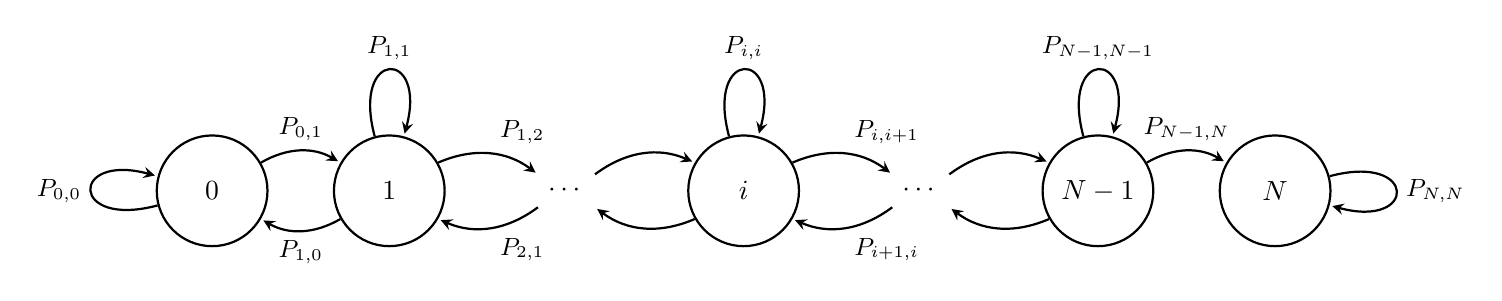
\begin{tikzpicture}[->,>=stealth,shorten >=1pt,auto,node distance=2.25cm,thick,main node/.style={scale=0.8, circle,draw,font=\sffamily\normalsize}]

                \node[circle, draw, minimum size = 40] (0) []{$0$};
                \node[circle, draw, minimum size = 40] (1) [right of = 0]{$1$};
                \node[]      (x) [right of = 1]{$\cdots$};
                \node[circle, draw, minimum size = 40] (2) [right of = x]{$i$};
                \node[]      (y) [right of = 2]{$\cdots$};
                \node[circle, draw, minimum size = 40] (3) [right of = y]{$N-1$};
                \node[circle, draw, minimum size = 40] (4) [right of = 3]{$N$};

                \path[every node/.style={font=\sffamily\small}]
                    (0) edge[loop left] node{$P_{0,0}$} (0)
                    (0) edge[bend left] node{$P_{0,1}$} (1)

                    (1) edge[loop above] node{$P_{1,1}$} (1)
                    (1) edge[bend left] node{$P_{1,2}$} (x)
                    (1) edge[bend left] node{$P_{1,0}$} (0)

                    (x) edge[bend left] (2)
                    (x) edge[bend left] node{$P_{2,1}$} (1)

                    (2) edge[loop above] node{$P_{i,i}$} (2)
                    (2) edge[bend left] node{$P_{i,i+1}$} (y)
                    (2) edge[bend left] (x)

                    (y) edge[bend left] (3)
                    (y) edge[bend left] node{$P_{i+1,i}$} (2)

                    (3) edge[loop above] node{$P_{N-1,N-1}$} (3)
                    (3) edge[bend left] node{$P_{N-1, N}$} (4)
                    (3) edge[bend left] (y)

                    (4) edge[loop right] node{$P_{N,N}$} (4)
                ;
            \end{tikzpicture}
        }
        \caption{The Markov model that studies convergence of Aloha-Q.}
    \end{figure}

    We move up one state -- from $i$ to $i+1$ -- when the current slot is unoccupied and only one hopping node trasmits in it. This implies that:
    \[P_{i,i+1} = \Pr[O_i = 0] \Pr[H_i = 1 \mid O_i = 0] = \rbk{\frac{N-i}{N}}^2 \rbk{\frac{N-1}{N}}^{N-i-1}\]
    
    where $O_i$ and $H_i$ are the r.v. that assert, respectively, if the slot is occupied, the number of hopping nodes transmitting and if the transmission occurred, all with respect to the number $i$ of currently occupied slots.

    We move down one state -- from $i$ to $i-1$ -- when the current slot is occupied and one or more hopping nodes transmit packets in it. This implies that:
    \[\begin{split}
        P_{i,i-1} &= \Pr[O_i = 1] \Pr[H_i \geq 1 \mid O_i = 1] \\
        &= \Pr[O_i = 1] (1-\Pr[H_i = 0 \mid O_i = 1]) \\
        &= \frac{i}{N} \rbk{1-\rbk{\frac{N-1}{N}}^{N-i}}
    \end{split} \]
    
    Lastly, we say in the same state -- from $i$ to $i$ -- when one of the following occurres:
    \begin{itemize}
        \item The current slot is occupied and no hopping nodes select the current slot.
        \item The current slot is unoccupied and two or more hopping nodes transmit packets in it.
        \item The current slot is unoccupied and there are no transmissions in it.
    \end{itemize}

    This implies that:
    \[\begin{split}
        P_{i,i} &= \Pr[O_i = 1] \Pr[H_i = 0 \mid O_i = 1] + \Pr[O_i = 0] \Pr[H_i \neq 1 \mid O_i = 0] \\
        &= \Pr[O_i = 1] \Pr[H_i = 0 \mid O_i = 1] + \Pr[O_i = 0] (1-\Pr[H_i = 1 \mid O_i = 0]) \\
        &= \frac{i}{N} \rbk{\frac{N-1}{N}}^{N-i} + \frac{N-i}{N}\rbk{1-\frac{N-i}{N} \rbk{\frac{N-1}{N}}^{N-i-1}}
    \end{split}\]

    To study convergence of the model, we consider the limit as $n \to +\infty$ of the power matrix $P^n$. We observe that for each $n \in \N$ the entries $P^n_{i,j}$ of the power matrix $P^n$ are given by:
    \[P_{i,j}^n = \sum_{m = 0}^N P^{n-1}_{i,m} P_{m,j} \]

    In other words, $P_{i,j}^n$ is the probability of reaching state $j$ starting from state $i$ through $n$ transitions. Threfore, to show that the protocol converges it suffices to show that, eventually, every node becomes steady and every slot becomes occupied:
    \[\lim_{n \to +\infty} P^n = \left [ \begin{matrix}
        0 & 0 & \cdots & 0 & 1 \\
        0 & 0 & \cdots & 0 & 1 \\
        \vdots & \ddots & \ddots & \ddots & \vdots \\ 
        0 & 0 & \cdots & 0 & 1 \\
        0 & 0 & \cdots & 0 & 1 \\
    \end{matrix}\right ]\]

    Indeed, this can be proven to be true. We omit the proof due to it requiring advanced linear algebra techniques, such as Jordan block analysis, Laplace expansions and Gershgoring discs.

    After proving that the scheme converges, we focus on the expected convergence time, i.e. the expected accumulated time the system spends in all states except state $N$, which is equal to the expected number of visits to these states across all $n \in \N$ steps, starting from state 0.
    \[\mathbb{E}[T] = \sum_{n = 1}^{+\infty} \sum_{j = 0}^{N-1} P^n_{0,j}\]

    \section{Performance of Aloha-Q}

    Experiments were conducted under the same assumptions used in the convergence analysis, with additional simulation parameters listed in \Cref{table}.

    \begin{figure}[H]
        \centering
        \begin{tabular}{ll}
            \hline
            Parameters & Values \\
            \hline
            Channel bit rate & 250 kbits/s \\
            Data packet length (simulation) & 1044 bits \\
            Data packet length (practical) & 935 bits \\
            ACK packet length (simulation) & 20 bits \\
            ACK packet length (practical) & 144 bits \\
            Slot length & 1100 bits \\
            \hline
        \end{tabular}
        \caption{Simulation parameters.}
        \label{table}
    \end{figure}
    
    \Cref{conv_time} illustrates the average convergence time for networks of varying sizes, where each data point represents the mean of 200 simulation runs. Convergence time is shown only up to 15 nodes, as this range is sufficient to demonstrate the close agreement between the analytical model and simulation results; beyond this point, theoretical computations become prohibitively complex. The expected convergence time involves extensive calculations as $n \to \infty$. To match this, very high values of $n$ are chose. For instance, $n = 10^9$ is used with $15$ nodes, ensuring that $P^n$ converges. The 95\% confidence interval for simulations with three nodes is approximately $\pm 3\%$, increasing to about $\pm 12\%$ for larger networks. These intervals are not shown in \Cref{conv_time} because they are nearly indistinguishable on the logarithmic $y$-axis.

    \begin{figure}[H]
        \centering
        \includegraphics[scale=0.75]{../images/conv_time.png}
        \caption{Average simulation convergence time.}
        \label{conv_time}
    \end{figure}
    
    To assess the impact of the learning rate, simulations were performed using several different values of this parameter, complemented by practical trials for validation. Each simulation curve represents the average of 100 runs, and each marker corresponds to the average of 50 practical trials. Networks containing 10, 20, and 200 nodes were simulated with an optimal frame size and a traffic load of 0.7 Erlangs. \Cref{cdf_conv_time} shows the Cumulative Density Function (CDF) of the convergence time of the networks with different number of nodes in the network. Each curve shows the results of 1000 simulations, 100 practical trials are implemented due to larger time cost.


    \begin{figure}[H]
        \centering
        \includegraphics[scale=0.75]{../images/cdf_conv_time.png}
        \caption{CDF of convergence time measured through analysis and simulation.}
        \label{cdf_conv_time}
    \end{figure}

    ALOHA-Q, Slotted ALOHA with exponential back-off, S-MAC, and Z-MAC were simulated in OPNET to evaluate and compare their performance in terms of throughput, end-to-end delay, and energy cost per bit of throughput. All protocols were tested in a network of 200 nodes, and ALOHA-Q (with the optimal frame size) was additionally simulated with 300 nodes to assess its performance under higher node density. Experiments using 20 IRIS nodes were also conducted to demonstrate throughput performance in practical network conditions. For S-MAC, a 10\% duty cycle was used, consistent with common practice. Each contention slot in Z-MAC was assigned a duration equivalent to 0.5 bits.

    \begin{figure}[H]
        \centering
        \includegraphics[scale=0.65]{../images/throughput.png}
        \caption{Real-time throughput.}
    \end{figure}

    \begin{figure}[H]
        \centering
        \includegraphics[scale=0.65]{../images/normalized_throughput.png}
        \caption{Normalized throughput.}
    \end{figure}

    \begin{figure}[H]
        \centering
        \includegraphics[scale=0.65]{../images/delay.png}
        \caption{End-to-end delay.}
    \end{figure}

    \begin{figure}[H]
        \centering
        \includegraphics[scale=0.65]{../images/energy.png}
        \caption{Energy cost per bit throughput.}
    \end{figure}


    \newpage
    \printbibliography
    \addcontentsline{toc}{section}{References}  % Add Bibliography to ToC
\end{document}